\section{Cơ sở lý thuyết và công nghệ}
\subsection{Cơ sở lý thuyết}
\subsubsection{Kiến trúc RESTful API}
\indent \indent RESTful API là một phong cách thiết kế API dành cho các hệ thống web, giúp đơn giản hóa việc quản lý và tương tác với các tài nguyên. Nó tập trung vào các tài nguyên hệ thống như tệp văn bản, hình ảnh, âm thanh, video hoặc dữ liệu động, với trạng thái của chúng được định dạng và truyền tải thông qua giao thức HTTP một cách hiệu quả.\\
\indent Các yếu tố chính trong RESTful API bao gồm:
\begin{itemize}
    \item[-] API (Application Programming Interface): Đây là bộ quy tắc và cơ chế cho phép một hệ thống hoặc thành phần tương tác với các hệ thống khác. API có thể trả về dữ liệu dưới dạng phổ biến như JSON hoặc XML.
    \item[-] REST (Representational State Transfer): Đây là một kiến trúc chuyển đổi cấu trúc dữ liệu, sử dụng các phương thức HTTP cơ bản như GET, POST, DELETE để giao tiếp giữa các thiết bị. Thay vì dùng URL để xử lý thông tin cụ thể, REST gửi yêu cầu HTTP đến URL nhằm thao tác dữ liệu.
\end{itemize}
\begin{figure}[H]
    \centering
    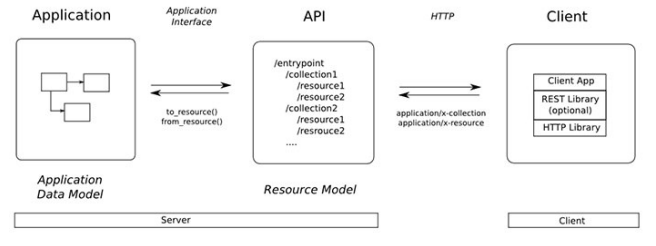
\includegraphics[width=0.7\textwidth]{Images/RESTful api.png}
    \vspace{15pt}
    \caption{Cách thức hoạt động của RESTful API}
\end{figure}
\indent \indent RESTful API được áp dụng rộng rãi trong thiết kế API cho web, giúp các hệ thống (web, mobile) kết nối và trao đổi dữ liệu một cách mượt mà. Ưu điểm chính của RESTful không quy định logic code hệ thống và không giới hạn bởi ngôn ngữ lập trình hệ thống, bất kỳ ngôn ngữ hoặc framework nào cũng có thể sử dụng để thiết kế một RESTful API.

\subsubsection{Mô hình Client - Server}
\indent \indent Mô hình Client-Server là một kiến trúc hệ thống phổ biến trong phát triển phần mềm, đặc biệt là các hệ thống web và di động. Trong mô hình này, hệ thống được chia thành hai phần chính: Client (máy khách) và Server (máy chủ). Client chịu trách nhiệm xử lý giao diện người dùng và gửi yêu cầu đến Server, trong khi Server xử lý logic kinh doanh, lưu trữ dữ liệu và trả về kết quả cho Client. Sự giao tiếp giữa hai bên thường diễn ra qua mạng, sử dụng các giao thức như HTTP hoặc HTTPS để đảm bảo an toàn và hiệu quả.\\
\indent Các thành phần chính của mô hình Client-Server bao gồm:
\begin{itemize}
    \item[-] Client: Là thiết bị hoặc hệ thống của người dùng cuối, chẳng hạn như trình duyệt web, hệ thống di động hoặc phần mềm máy tính. Client thu thập đầu vào từ người dùng, gửi yêu cầu đến Server và hiển thị kết quả nhận được. Trong đồ án này, phần frontend được xây dựng bằng ReactJS với TypeScript đóng vai trò là Client, cho phép người dùng tương tác như tìm kiếm sự kiện, mua vé hoặc chat.
    \item[-] Server: Là máy chủ trung tâm, xử lý các yêu cầu từ Client, thực hiện các tác vụ phức tạp như xác thực, truy vấn cơ sở dữ liệu và tính toán logic. Server trả về dữ liệu dưới dạng phù hợp, thường là JSON qua API. Trong hệ thống MyTicket, backend sử dụng Node.js làm Server, kết nối với MongoDB để quản lý dữ liệu sự kiện và vé.
    \item[-] Giao tiếp: Client gửi yêu cầu (request) đến Server qua mạng, và Server phản hồi (response) với dữ liệu cần thiết. Mô hình này hỗ trợ mở rộng bằng cách thêm nhiều Client mà không ảnh hưởng đến Server, đồng thời cho phép Server được nâng cấp độc lập.
\end{itemize}
\begin{figure}[H]
    \centering
    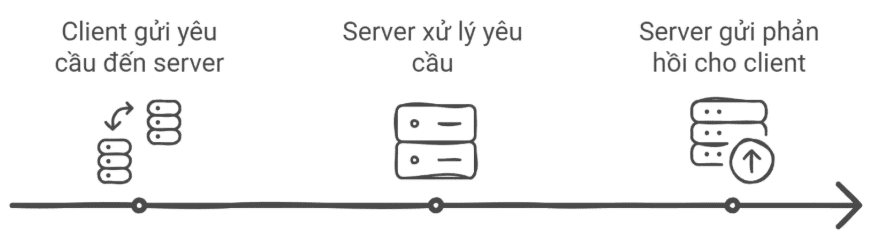
\includegraphics[width=0.7\textwidth]{Images/MoHinhClient_Server.png}
    \vspace{15pt}
    \caption{Cách thức hoạt động của mô hình Client-Server}
\end{figure}
\indent \indent Ưu điểm của mô hình Client-Server:
\begin{itemize}
    \item[-] Tập trung hóa quản lý: Dữ liệu và logic chính được lưu trữ trên Server, dễ dàng bảo trì và cập nhật mà không cần thay đổi Client.
    \item[-] Khả năng mở rộng: Hỗ trợ nhiều người dùng đồng thời, phù hợp với hệ thống như đặt vé sự kiện nơi lượng truy cập có thể tăng đột biến.
    \item[-] Bảo mật cao hơn: Server có thể kiểm soát quyền truy cập, mã hóa dữ liệu và bảo vệ khỏi các rủi ro từ phía Client.
    \item[-] Hiệu quả tài nguyên: Client chỉ cần xử lý giao diện, trong khi Server đảm nhận các tác vụ nặng, giúp tối ưu hóa hiệu suất hệ thống.
\end{itemize}
\indent \indent Tuy nhiên, mô hình này cũng có nhược điểm như phụ thuộc vào kết nối mạng ổn định và có thể gặp tình trạng quá tải Server nếu không thiết kế tốt.

\subsubsection{Cơ sở dữ liệu dữ liệu}
\indent \indent Cơ sở dữ liệu (Database) hay gọi tắt là CSDL, là tập hợp có tổ chức của các dữ liệu liên quan logic với nhau, được lưu trữ và truy cập từ hệ thống máy tính nhằm phục vụ nhu cầu khai thác thông tin của người dùng hoặc hệ thống. Trong thực tế, khái niệm này thường bao quát cả hệ quản trị cơ sở dữ liệu (DBMS) và hệ thống cơ sở dữ liệu tổng thể. 
\begin{figure}[H]
    \centering
    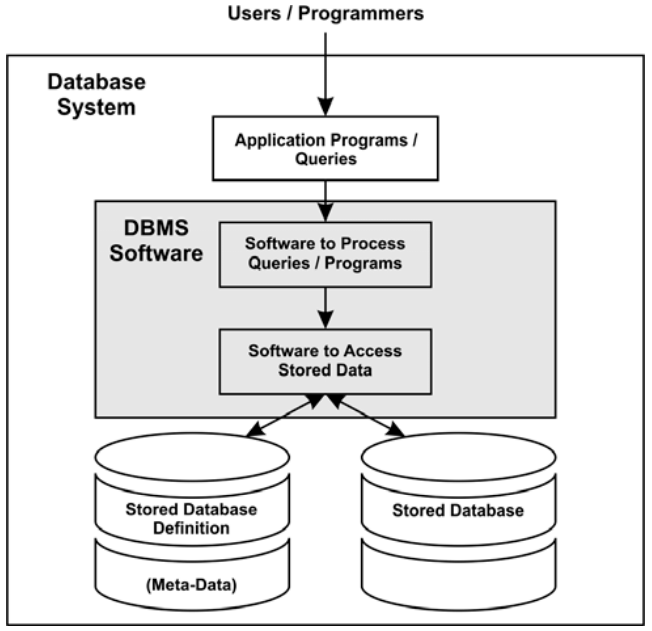
\includegraphics[width=0.7\textwidth]{Images/CSDL.png}
    \vspace{15pt}
    \caption{Hệ thống cơ sở dữ liệu đơn giản}
\end{figure}
\indent Hệ thống cơ sở dữ liệu bao gồm các thành phần chính:
\begin{table}[H]
\centering
\renewcommand{\arraystretch}{1.3}
\setlength{\tabcolsep}{6pt}
\begin{tabularx}{\textwidth}{|p{4cm}|X|}
\hline
\multicolumn{2}{|c|}{\textbf{A. Người dùng và Vai trò}} \\
\hline
\textbf{Thành phần} & \textbf{Vai trò/Mô tả} \\
\hline
\textbf{Người dùng} & Là những người tương tác trực tiếp với dữ liệu thông qua hệ thống, thực hiện các thao tác cơ bản như thêm, xóa, chỉnh sửa (CRUD) hoặc truy vấn dữ liệu. \\
\hline
\textbf{Người Phát triển Hệ thống} & Bao gồm Phân tích viên Hệ thống (xác định yêu cầu) và Lập trình viên (viết mã hệ thống và truy vấn). Họ xây dựng các chương trình để người dùng có thể truy cập CSDL. \\
\hline
\textbf{Người Quản trị CSDL (DBA)} & Là người có quyền điều khiển tập trung cao nhất. Họ chịu trách nhiệm thiết kế, triển khai, bảo trì, cấp quyền và đảm bảo tính bảo mật/toàn vẹn cho toàn bộ CSDL và các chương trình truy xuất nó. \\
\hline
\multicolumn{2}{|c|}{\textbf{B. Phần mềm và Giao diện}} \\
\hline
\textbf{Hệ Quản trị Cơ sở Dữ liệu (DBMS)} & Là phần mềm trung tâm của hệ thống. Chức năng chính là tạo, duy trì và cung cấp cơ chế truy cập có kiểm soát (bảo mật, đồng thời) đến dữ liệu. \\
\hline
\textbf{hệ thống} & Là các chương trình giao tiếp (phần mềm) được phát triển để người dùng cuối có thể truy cập và tương tác với dữ liệu một cách dễ dàng và có cấu trúc. \\
\hline
\textbf{Giao diện Người dùng} & Là các phương tiện hiển thị (ví dụ: màn hình nhập liệu, form, báo cáo) cho phép người dùng thao tác với các thành phần của hệ thống CSDL. \\
\hline
\multicolumn{2}{|c|}{\textbf{C. Dữ liệu và Lưu trữ}} \\
\hline
\textbf{Cơ sở Dữ liệu (CSDL)} & Là tập hợp dữ liệu có liên quan logic với nhau, được tổ chức và lưu trữ nhằm phục vụ nhu cầu thông tin chung của nhiều người dùng trong một tổ chức. \\
\hline
\textbf{Dữ liệu} & Là thông tin thực tế liên quan đến hệ thống (ví dụ: tên khách hàng, mã sản phẩm) được lưu trữ dưới dạng các tập tin trên thiết bị vật lý. \\
\hline
\textbf{Hệ thống Chủ} & Là hệ thống máy tính vật lý hoặc máy chủ, có trách nhiệm quản lý và thực hiện việc truy cập vật lý đến các tập tin chứa dữ liệu. \\
\hline
\end{tabularx}
\vspace{15pt} % Thêm khoảng cách nếu cần thiết để tách bảng và caption
\caption{Các Thành phần Chính của Hệ thống Cơ sở Dữ liệu}
\label{tab:dbs_components}
\end{table}
Về phân loại, có 2 loại cơ sở dữ liệu khác nhau là Cở sở dữ liệu quan hệ (Relational Database) và Cơ sở dữ liệu phi quan hệ (NoSQL Database). Bảng dưới đây là những tiêu chí so sánh sự khác nhau giữa chúng:
\begin{table}[H]
\centering
\renewcommand{\arraystretch}{1.3} % Giảm arraystretch một chút để phù hợp với X (1.5 có thể làm giãn quá mức)
\setlength{\tabcolsep}{6pt}
\begin{tabularx}{\textwidth}{|l|X|X|}
\hline
\textbf{Tiêu chí} & \textbf{CSDL Quan hệ (SQL)} & \textbf{CSDL Phi quan hệ (NoSQL)} \\ \hline
\textbf{Định nghĩa} & Đây là loại cơ sở dữ liệu thường gọi là RDBMS, tập trung vào việc tổ chức dữ liệu theo mối quan hệ giữa các bảng. & Đây là loại cơ sở dữ liệu thường được xem như không quan hệ hoặc phân tán, không dựa vào cấu trúc bảng cố định. \\ \hline
\textbf{Mục đích sử dụng} & Dùng ngôn ngữ SQL để phân tích dữ liệu, giúp rút ra insights sâu hơn, thường áp dụng trong OLAP để xử lý phân tích dữ liệu lớn. & Được thiết kế để đáp ứng nhu cầu của các hệ thống hiện đại, như xử lý dữ liệu thời gian thực hoặc khối lượng lớn. \\ \hline
\textbf{Mô hình lưu trữ} & Dữ liệu được sắp xếp theo dạng bảng với hàng và cột rõ ràng. & Dữ liệu có thể lưu dưới dạng tài liệu, cặp khóa-giá trị, hoặc biểu đồ. \\ \hline
\textbf{Schema} & Yêu cầu schema được định nghĩa sẵn từ đầu (schema-rigid), đảm bảo cấu trúc dữ liệu nhất quán. & Sử dụng schema động (schema-less), phù hợp với dữ liệu không cấu trúc hoặc thay đổi thường xuyên. \\ \hline
\textbf{Khả năng mở rộng} & Mở rộng theo chiều dọc (Vertical Scaling), nghĩa là nâng cấp phần cứng của máy chủ hiện tại. & Mở rộng theo chiều ngang (Horizontal Scaling), dễ dàng thêm nhiều máy chủ để phân tải. \\ \hline
\textbf{Ví dụ} & Một số hệ phổ biến như Oracle, PostgreSQL, MySQL hay MS SQL Server. & Các ví dụ điển hình bao gồm MongoDB (Document), Redis (Key-Value), Neo4j (Graph), Cassandra và HBase. \\ \hline
\textbf{Lưu trữ dữ liệu phân cấp} & Không lý tưởng cho dữ liệu phân cấp, vì khó xử lý các mối quan hệ phức tạp. & Rất phù hợp cho dữ liệu phân cấp nhờ mô hình cặp khóa-giá trị, giúp truy xuất nhanh. \\ \hline
\textbf{Năm phát triển} & Ra đời vào thập niên 1970 để giải quyết hạn chế của lưu trữ file phẳng. & Phát triển mạnh vào cuối những năm 2000, nhằm khắc phục nhược điểm của SQL trong hệ thống hiện đại. \\ \hline
\textbf{Tính nhất quán} & Đảm bảo nhất quán mạnh mẽ (Strong Consistency), tránh lỗi dữ liệu. & Tùy thuộc vào hệ thống; ưu tiên nhất quán cuối cùng (Eventual Consistency) để tăng hiệu suất và khả năng mở rộng. \\ \hline
\textbf{Network} & Thường dùng mạng cao cấp như Infiniband hoặc Fabric Path để đảm bảo hiệu suất. & Sử dụng mạng thông thường như Ethernet, dễ triển khai hơn. \\ \hline
\textbf{Loại lưu trữ} & Ưu tiên lưu trữ cao cấp như SAN hoặc RAID để bảo vệ dữ liệu. & Dùng ổ đĩa thông thường như HDD chuẩn hoặc JBOD, tiết kiệm chi phí. \\ \hline
\textbf{Hiệu suất} & Tốt nếu thiết kế CSDL tối ưu, nhưng có thể chậm nếu cần JOIN phức tạp. & Thường nhanh hơn nhờ denormalization, cho phép lấy dữ liệu một cách trực tiếp mà không cần JOIN phức tạp. \\ \hline
\end{tabularx}
\vspace{15pt}
\caption{So sánh Cơ sở Dữ liệu Quan hệ (SQL) và Phi quan hệ (NoSQL)}
\label{tab:sql_vs_nosql}
\end{table}
\subsubsection{Xác thực và Phân quyền người dùng (Authentication \& Authorization)}
\indent \indent \textbf{a) Xác thực (Authentication)}\\
\indent Xác thực là quá trình kiểm tra và xác nhận danh tính của người dùng hoặc thiết bị trước khi cho phép truy cập vào hệ thống. Mục tiêu chính là đảm bảo rằng người dùng là chính họ, dựa trên thông tin họ cung cấp như tên đăng nhập, mật khẩu, mã OTP hoặc các phương pháp sinh trắc học. \\
\indent Quá trình xác thực thường bao gồm các bước sau:
\begin{itemize}
    \item[1.] Người dùng nhập thông tin đăng nhập (ví dụ: email và mật khẩu).
    \item[2.] Hệ thống so sánh thông tin này với dữ liệu đã lưu trữ trong cơ sở dữ liệu.
    \item[3.] Nếu thông tin khớp, hệ thống tạo một phiên làm việc (session) hoặc token (như JWT - JSON Web Token) để xác nhận danh tính trong các yêu cầu tiếp theo.
\end{itemize}
\indent \indent Các phương pháp xác thực phổ biến bao gồm:
\begin{itemize}
    \item[-] Xác thực bằng mật khẩu: Phương pháp cơ bản nhưng cần mã hóa (như bcrypt) để tăng tính bảo mật.
    \item[-] Xác thực hai yếu tố (2FA): Kết hợp mật khẩu với mã OTP gửi qua SMS hoặc hệ thống, nâng cao an toàn.
    \item[-] Xác thực bằng token: Sử dụng token không đổi (refresh token) và token truy cập (access token) để quản lý phiên làm việc.
\end{itemize}
\indent \indent \textbf{b) Phân quyền (Authorization)}\\
\indent Phân quyền là quá trình xác định quyền hạn của người dùng đã được xác thực, quyết định họ có thể thực hiện những hành động nào trong hệ thống. \\
\indent Phân quyền thường dựa trên:
\begin{itemize}
    \item[-] Vai trò (Role-Based Access Control - RBAC): Gán quyền theo vai trò, ví dụ quản trị viên có quyền chỉnh sửa sự kiện, trong khi người dùng chỉ xem thông tin.
    \item[-] Quy tắc (Rule-Based Access Control): Áp dụng các quy định cụ thể, như chỉ cho phép mua vé khi sự kiện còn chỗ.
    \item[-] Danh sách kiểm soát truy cập (ACL): Xác định quyền dựa trên danh sách người dùng hoặc nhóm.
\end{itemize}
\indent \indent Sự kết hợp giữa xác thực và phân quyền giúp hệ thống đảm bảo an toàn, bảo mật thông tin và cung cấp trải nghiệm cá nhân hóa cho từng loại người dùng.

\subsubsection{Thuật toán LightGBM Ranker (LambdaRank – Gradient Boosted Decision Trees for Ranking)}
\indent \indent LightGBM (Light Gradient Boosting Machine) là một framework mã nguồn mở được phát triển bởi Microsoft, dựa trên thuật toán gradient boosting. Ra mắt vào năm 2016, LightGBM được thiết kế để tối ưu hiệu suất và tốc độ xử lý trên các tập dữ liệu lớn, với khả năng hỗ trợ nhiều loại bài toán như phân loại, hồi quy và đặc biệt là xếp hạng (ranking).\\
\indent LightGBM Ranker là một biến thể của LightGBM được thiết kế cho bài toán \textbf{Learning to Rank (LTR)}, một nhánh của máy học tập trung vào việc sắp xếp các đối tượng theo thứ tự phù hợp dựa trên độ liên quan. Trong LightGBM Ranker, hàm mất mát LambdaRank thường được sử dụng để tối ưu hóa trực tiếp các chỉ số đánh giá xếp hạng như \textbf{NDCG (Normalized Discounted Cumulative Gain).}\\
\indent Nguyên lý hoạt động:
\begin{itemize}
    \item[-] Gradient Boosting: LightGBM xây dựng một chuỗi các cây quyết định nông (shallow trees) theo cách thức boosting, trong đó mỗi cây tiếp theo học từ phần sai sót (residual) của các cây trước đó.
    \item[-] Pairwise Ranking: Thay vì dự đoán nhãn tuyệt đối, LambdaRank học thứ tự tương đối giữa các cặp item. Mô hình được huấn luyện để phân biệt item nào nên được xếp hạng cao hơn item khác trong cùng một nhóm (ví dụ: cùng một người dùng).
    \item[-] Lambda Gradient: Đạo hàm của hàm mất mát được tính dựa trên sự thay đổi của chỉ số NDCG khi hoán đổi thứ tự hai item, từ đó xác định hướng tối ưu cho việc cập nhật trọng số của mô hình.
    \item[-] Leaf-wise Tree Growth: Khác với các thuật toán boosting truyền thống sử dụng chiến lược phát triển cây theo chiều sâu (depth-wise), LightGBM sử dụng chiến lược phát triển theo lá (leaf-wise), chọn lá có độ lợi thông tin cao nhất để phân chia, giúp tăng tốc độ huấn luyện và cải thiện độ chính xác.
\end{itemize}
% \begin{figure}[H]
%     \centering
%     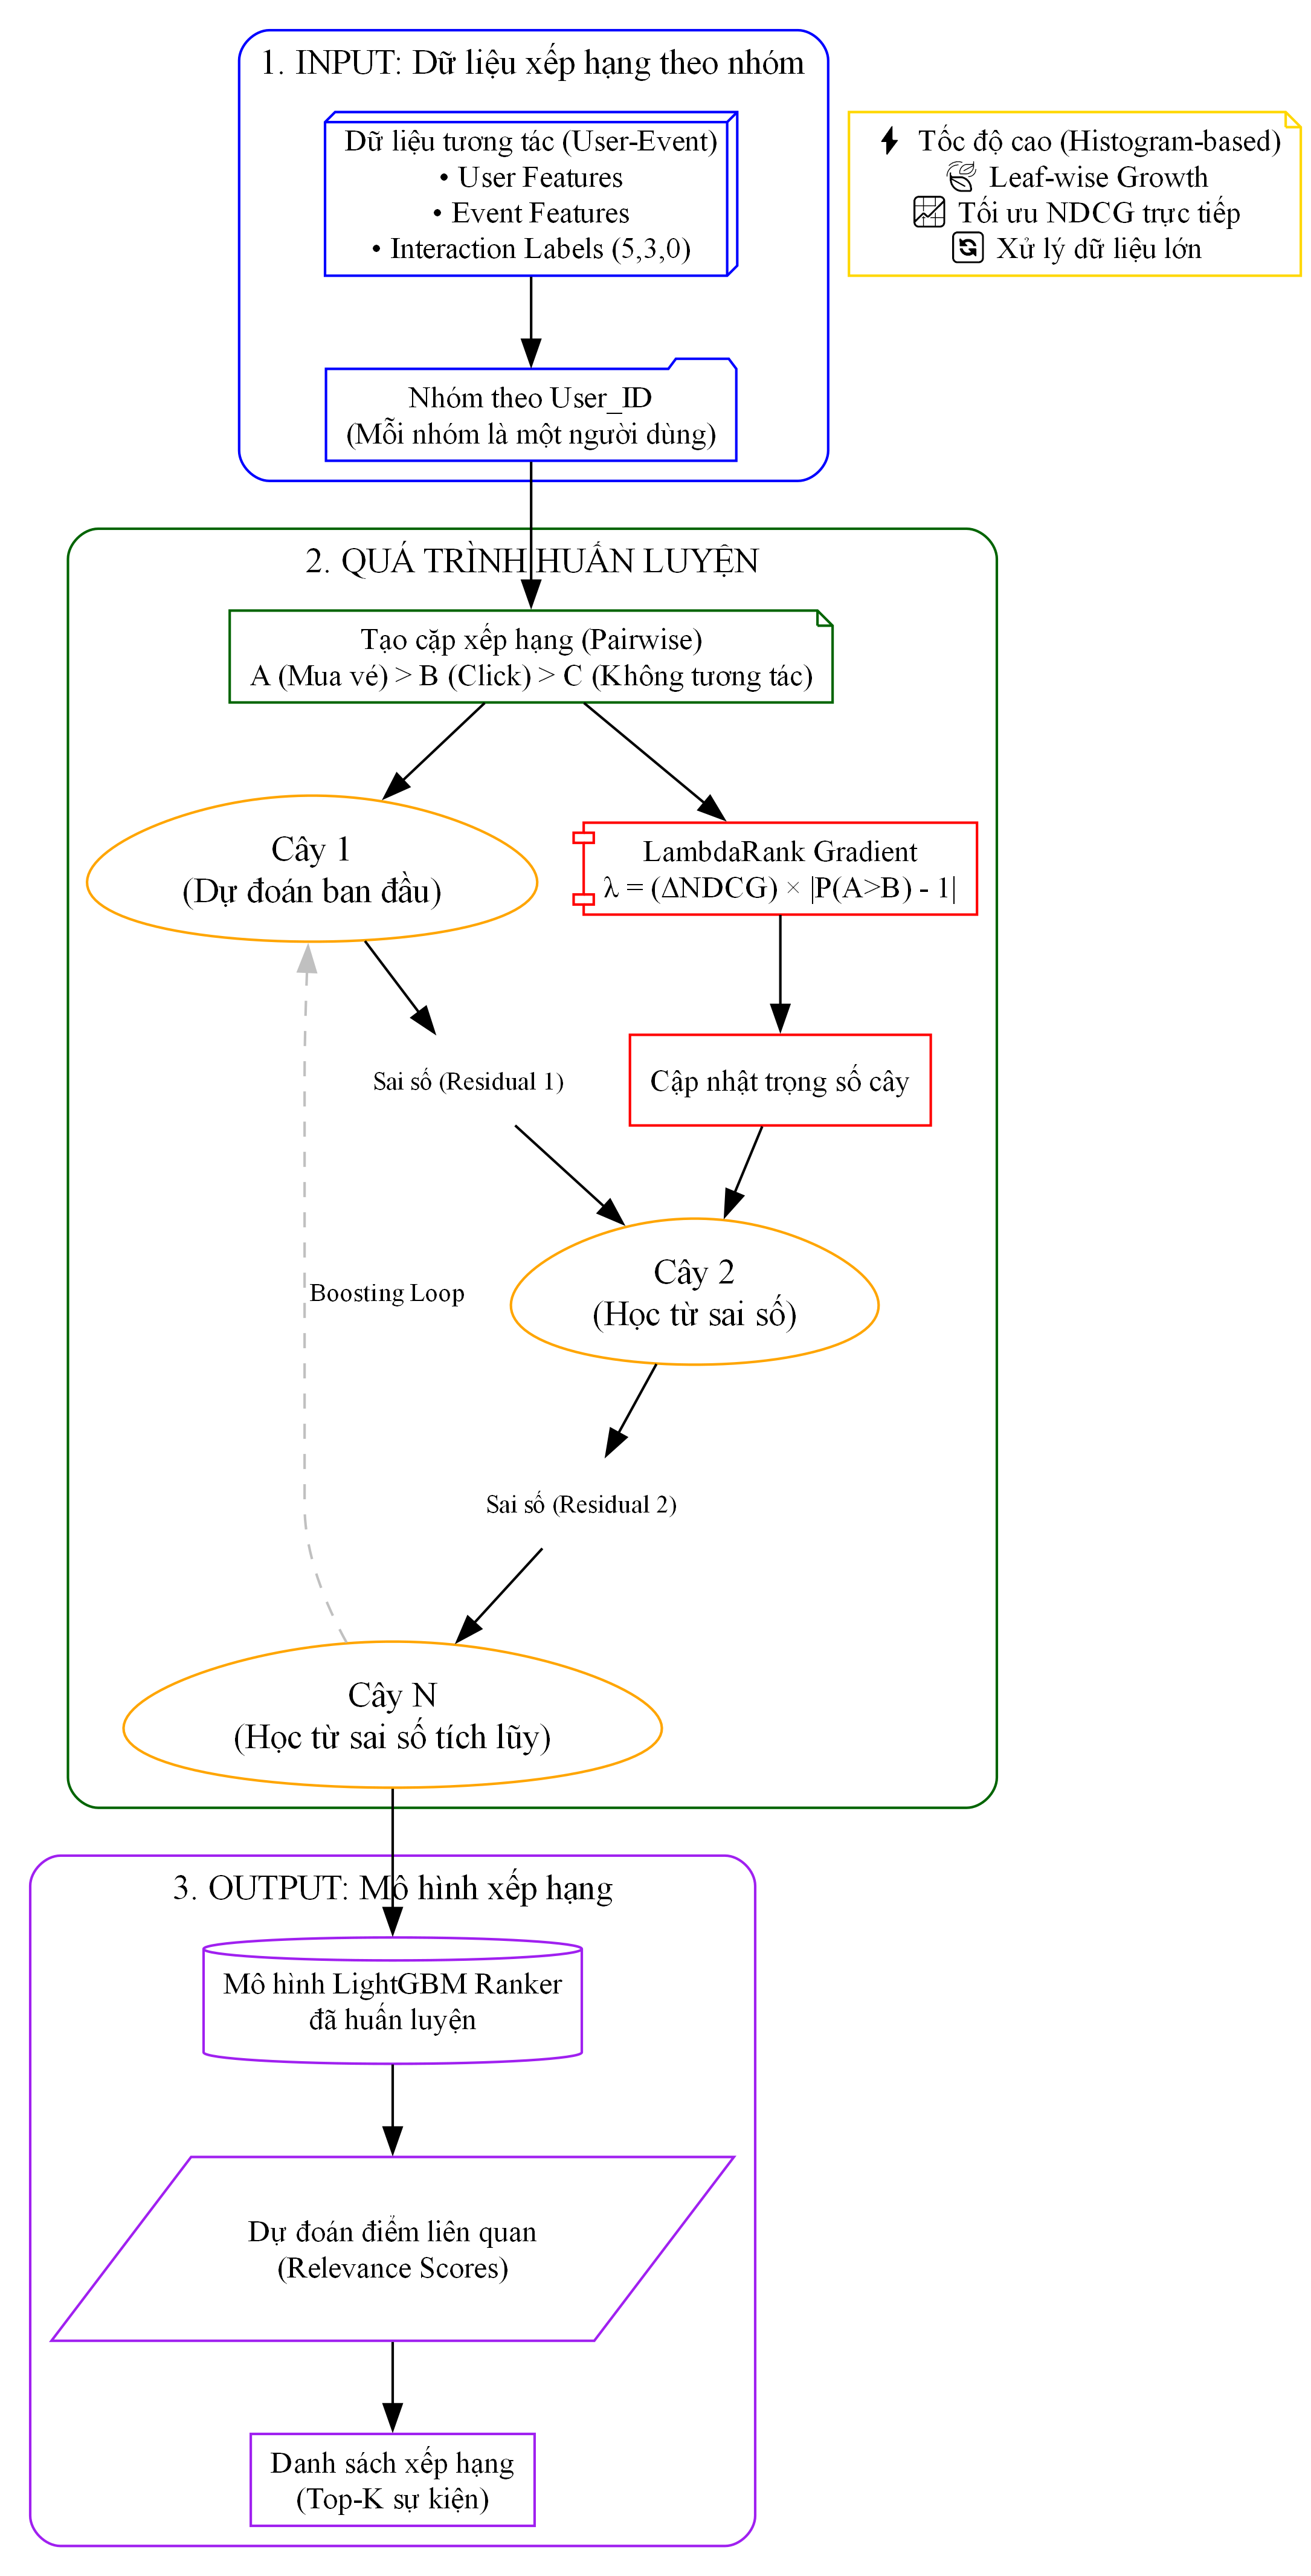
\includegraphics[width=0.72\textwidth]{Images/lightgbm_ranker_lambdarank.png}
%     \vspace{15pt}
%     \caption{Sơ đồ minh họa Thuật toán LightGBM Ranker (LambdaRank)}
% \end{figure}
\indent \indent Công dụng chính của LightGBM Ranker là giải quyết các bài toán yêu cầu sắp xếp thứ tự dựa trên độ liên quan, chẳng hạn như hệ thống đề xuất, tìm kiếm thông tin và xếp hạng sản phẩm. Nhờ vào tốc độ xử lý nhanh, khả năng mở rộng và hỗ trợ dữ liệu lớn, LightGBM Ranker đã trở thành một trong những lựa chọn phổ biến trong các hệ thống xếp hạng quy mô công nghiệp.

\subsection{Công nghệ sử dụng}
\subsubsection{TypeScript}
\begin{figure}[H]
    \centering
    
\includegraphics[width=0.2\textwidth]{Images/Typescript.png}
    \vspace{15pt}
    \caption{Ngôn ngữ lập trình TypeScript}
\end{figure}
\indent \indent TypeScript là một ngôn ngữ lập trình mã nguồn mở do Microsoft phát triển. Nó được xem là một siêu tập hợp (superset) của JavaScript (JS), nghĩa là mọi mã JS hợp lệ đều là mã TypeScript hợp lệ. Điểm mạnh lớn nhất của TypeScript là việc bổ sung kiểu dữ liệu tĩnh (static typing) vào JavaScript, giúp lập trình viên viết mã an toàn và dễ bảo trì hơn.

Mã TypeScript (\texttt{.ts}) không thể chạy trực tiếp trên trình duyệt mà cần được biên dịch (compile) thành mã JavaScript thuần túy để có thể hoạt động ở mọi nơi mà JS được hỗ trợ (trình duyệt, máy chủ Node.js, v.v.).

\indent TypeScript mang lại nhiều cải tiến đáng kể trong quy trình phát triển:
\begin{itemize}
    \item[-] Phát Hiện Lỗi Sớm Hơn: Nhờ có kiểu dữ liệu tĩnh, TypeScript giúp bạn tìm thấy các lỗi phổ biến ngay trong quá trình viết mã (chứ không phải khi chạy chương trình). Điều này giúp tiết kiệm thời gian gỡ lỗi và làm tăng chất lượng mã nguồn.
    \item[-] Xây Dựng hệ thống Lớn Dễ Dàng: Với cấu trúc rõ ràng, hỗ trợ lập trình hướng đối tượng (OOP) và khả năng quản lý mã nguồn tốt hơn, TypeScript là lựa chọn lý tưởng cho các dự án quy mô lớn, nơi mà sự rõ ràng và khả năng bảo trì là tối quan trọng.
    \item[-] Tương Thích Ngược Và Tiến:
    \begin{itemize}
        \item[+] Hỗ trợ JS Hiện Đại: TypeScript cho phép bạn sử dụng các tính năng mới nhất của JavaScript (như ECMAScript 2015/ES6 trở lên) và biên dịch chúng về phiên bản JS cũ hơn, đảm bảo khả năng chạy trên nhiều môi trường khác nhau.
        \item[+] Là JavaScript (Về Bản Chất): Vì cuối cùng được biên dịch thành JS, mã TypeScript có thể chạy ở bất cứ đâu. Hơn nữa, bạn có thể kết hợp mã JS hiện có vào dự án TS một cách dễ dàng, giúp việc chuyển đổi và tiếp cận trở nên linh hoạt.
    \end{itemize}
    \item[-] Được Cộng Đồng Và Framework Ưu Ái:
    \begin{itemize}
        \item[+] Mã Nguồn Mở \& Miễn Phí: TypeScript là dự án mã nguồn mở nên bạn có thể sử dụng hoàn toàn miễn phí, đi kèm với sự hỗ trợ lớn từ cộng đồng.
        \item[+] Hỗ Trợ Từ Framework: Các Framework JavaScript phổ biến hiện nay (như Angular, React và Vue) đều có sự hỗ trợ mạnh mẽ và thậm chí khuyến khích sử dụng TypeScript làm ngôn ngữ chính.
    \end{itemize}
\end{itemize}
\indent \indent Tóm lại, TypeScript mang lại sự ổn định, rõ ràng và hiệu quả cho việc phát triển web hiện đại. Nó là cầu nối giúp lập trình viên tận dụng được sự linh hoạt của JavaScript đồng thời có được sự an toàn của kiểu dữ liệu tĩnh.
\subsubsection{ReactJS}
\begin{figure}[H]
    \centering
    
\includegraphics[width=0.2\textwidth]{Images/react.png}
    \vspace{15pt}
    \caption{Thư viên ReactJS}
\end{figure}
\indent \indent ReactJS (thường được gọi là React) là một thư viện JavaScript mã nguồn mở, được phát triển và bảo trì bởi Meta (trước đây là Facebook). React ra đời với mục đích chính là giải quyết các thách thức trong việc xây dựng giao diện người dùng (User Interface - UI) động, phức tạp và có hiệu suất cao, đặc biệt là cho các hệ thống web một trang (Single Page Applications - SPAs).

Triết lý cốt lõi của React là xây dựng giao diện người dùng thông qua việc "lắp ráp" các thành phần (Components). Mỗi thành phần là một khối giao diện độc lập (ví dụ: một nút bấm, một thanh tìm kiếm, một thẻ thông tin người dùng), tự quản lý trạng thái (state) của riêng nó và có thể được tái sử dụng trong toàn bộ hệ thống.

React đã trở thành một trong những công nghệ front-end phổ biến nhất trên toàn cầu nhờ vào những ưu điểm kỹ thuật vượt trội sau:
\begin{itemize}
    \item[-] Hiệu suất cao (Nhờ Virtual DOM): React tạo ra một bản sao "ảo" của giao diện. Khi dữ liệu thay đổi, nó chỉ cập nhật những chi tiết nhỏ cần thiết trên giao diện thật, thay vì tải lại toàn bộ, giúp hệ thống chạy cực kỳ nhanh và mượt.
    \item[-] Kiến trúc dựa trên Thành phần (Components): React chia giao diện thành các khối nhỏ, độc lập (như khối LEGO). Điều này giúp code rất dễ tái sử dụng, dễ quản lý, và dễ dàng sửa lỗi mà không ảnh hưởng đến các phần khác.
    \item[-] Cú pháp Khai báo (Declarative UI): Người dùng chỉ cần "ra lệnh" cho React biết giao diện nên trông như thế nào ở các trạng thái khác nhau. React sẽ tự lo phần còn lại. Cách này giúp code dễ đọc, dễ hiểu và dễ dự đoán hơn.
    \item[-] Cộng đồng lớn và Hệ sinh thái mạnh: React có một cộng đồng khổng lồ, đồng nghĩa với việc có rất nhiều tài liệu, khóa học, và các thư viện hỗ trợ (như Redux, React Router) để giải quyết hầu hết mọi vấn đề.
    \item[-] "Học một lần, viết mọi nơi": Khi đã thành thạo React, lập trình viên thể dễ dàng sử dụng kiến thức đó để xây dựng hệ thống di động (iOS và Android) với React Native, giúp tiết kiệm rất nhiều thời gian và nguồn lực.
\end{itemize}
\subsubsection{NodeJS}
\begin{figure}[H]
    \centering
    
\includegraphics[width=0.3\textwidth]{Images/nodejs.png}
    \vspace{15pt}
    \caption{Môi trường lập trình NodeJS}
\end{figure}
\indent \indent Nodejs là một nền tảng phát triển hệ thống phía máy chủ, cho phép lập trình viên sử dụng JavaScript để xây dựng các hệ thống web nhanh chóng và hiệu quả. Với kiến trúc phi đồng bộ và sự kiện, Node.js rất phù hợp cho các hệ thống cần xử lý nhiều kết nối đồng thời, chẳng hạn như hệ thống trò chuyện hoặc dịch vụ phát trực tuyến. 
NodeJS cũng nổi bật với hệ sinh thái phong phú của các thư viện và công cụ, giúp tăng tốc quá trình phát triển và tối ưu hóa hiệu suất của hệ thống.
\begin{itemize}
    \item[-] Hiệu suất cao nhờ mô hình phi đồng bộ: NodeJS sử dụng kiến trúc I/O không chặn (non-blocking I/O) và một Vòng lặp Sự kiện (Event Loop). Thay vì "chờ" một tác vụ (như truy vấn cơ sở dữ liệu) hoàn tất và làm nghẽn luồng xử lý, NodeJS sẽ ủy thác tác vụ đó và tiếp tục xử lý các yêu cầu khác. Khi tác vụ hoàn tất, nó sẽ thông báo lại qua cơ chế callback (hoặc Promise/Async-Await). Điều này cho phép NodeJS xử lý hàng nghìn kết nối đồng thời một cách hiệu quả chỉ với một luồng, tối ưu hóa việc sử dụng tài nguyên hệ thống.
    \item[-] Chạy trên nhiều nền tảng (cross-platform): Mã nguồn của NodeJS có khả năng chạy nhất quán trên nhiều hệ điều hành phổ biến, bao gồm Windows, macOS và các bản phân phối Linux. Khả năng này loại bỏ sự khác biệt về môi trường, cho phép các nhà phát triển xây dựng hệ thống trên máy cá nhân và triển khai lên máy chủ một cách liền mạch mà không cần sửa đổi mã nguồn.
    \item[-] Hệ sinh thái npm phong phú với hàng triệu gói thư viện: NPM (Node Package Manager) là kho lưu trữ các gói phần mềm (packages) và thư viện mã nguồn mở lớn nhất thế giới. Nó hoạt động như một trình quản lý phụ thuộc, cho phép các nhà phát triển dễ dàng tìm, cài đặt và tái sử dụng các mô-đun cho gần như mọi chức năng. Điều này giúp tăng tốc đáng kể quá trình phát triển và đảm bảo chất lượng thông qua việc sử dụng các giải pháp đã được cộng đồng kiểm chứng.
    \item[-] Dễ dàng tích hợp với các dịch vụ và API của bên thứ ba: Nhờ bản chất phi đồng bộ, NodeJS rất lý tưởng để xây dựng các hệ thống trung gian (như API Gateway) trong kiến trúc Microservices. Nó có thể thực hiện nhiều lệnh gọi API đến các dịch vụ bên ngoài một cách song song mà không làm chậm thời gian phản hồi chung của hệ thống, giúp tối ưu hóa việc tổng hợp dữ liệu từ nhiều nguồn.
    \item[-] Cộng đồng hỗ trợ lớn và tài liệu phong phú: NodeJS sở hữu một cộng đồng toàn cầu cực kỳ lớn mạnh và năng động, được hậu thuẫn bởi OpenJS Foundation và nhiều tập đoàn công nghệ lớn. Điều này đảm bảo rằng tài liệu, các bài hướng dẫn và các diễn đàn hỗ trợ (như Stack Overflow) luôn có sẵn, giúp giải quyết vấnE đề kỹ thuật nhanh chóng và đảm bảo nền tảng được cập nhật, bảo trì liên tục.
\end{itemize}

\subsubsection{Ngôn ngữ lập trình Python}
\begin{figure}[H]
    \centering
    
\includegraphics[width=0.2\textwidth]{Images/python.png}
    \vspace{15pt}
    \caption{Ngôn ngữ lập trình Python}
\end{figure}
\indent \indent Python là một ngôn ngữ lập trình bậc cao, được Guido van Rossum tạo ra và lần đầu ra mắt vào năm 1991. Ngôn ngữ này được thiết kế với triết lý ưu tiên tính dễ đọc, cú pháp rõ ràng và ngắn gọn, giúp lập trình viên có thể viết mã dễ hiểu và dễ bảo trì. Python hỗ trợ nhiều mô hình lập trình như lập trình hướng đối tượng, lập trình cấu trúc và lập trình hàm, làm cho nó trở thành một công cụ linh hoạt trong nhiều lĩnh vực.\\
\indent Trong lĩnh vực máy học và khoa học dữ liệu, Python đã trở thành ngôn ngữ hàng đầu nhờ hệ sinh thái thư viện phong phú và mạnh mẽ. Các thư viện như NumPy và Pandas cung cấp khả năng xử lý dữ liệu số và cấu trúc dữ liệu hiệu quả, trong khi Scikit-learn cung cấp các công cụ toàn diện cho việc xây dựng và đánh giá mô hình máy học. Đối với các bài toán học sâu, các framework như TensorFlow và PyTorch cho phép triển khai các mạng neural phức tạp. Ngoài ra, các thư viện chuyên biệt cho bài toán xếp hạng và gradient boosting như LightGBM, XGBoost và CatBoost cũng được tích hợp dễ dàng trong Python. \\
\indent Lợi ích chính của Python trong máy học bao gồm:
\begin{itemize}
    \item[-] Dễ học và dễ sử dụng: Cú pháp trực quan giúp lập trình viên tập trung vào giải thuật thay vì chi tiết cú pháp.
    \item[-] Tính linh hoạt cao: Python có thể được sử dụng ở mọi giai đoạn của pipeline máy học, từ tiền xử lý dữ liệu, huấn luyện mô hình đến triển khai sản phẩm.
    \item[-] Cộng đồng và tài nguyên phong phú: Với số lượng người dùng lớn, Python có hệ sinh thái thư viện phát triển nhanh chóng, cùng nhiều tài liệu hướng dẫn, diễn đàn hỗ trợ và các khóa học trực tuyến.
    \item[-] Khả năng tích hợp đa nền tảng: Python có thể kết nối với nhiều hệ thống và ngôn ngữ khác, hỗ trợ đọc và xuất dữ liệu dưới nhiều định dạng, đồng thời dễ dàng triển khai dưới dạng dịch vụ web thông qua các framework như Flask hoặc FastAPI.
\end{itemize}

\subsubsection{MongoDB}
\begin{figure}[H]
    \centering
    
\includegraphics[width=0.35\textwidth]{Images/mongoDB.png}
    \vspace{15pt}
    \caption{Hệ quản trị cơ sở dữ liệu MongoDB}
\end{figure}
\indent \indent MongoDB được khởi nguồn từ công ty 10gen (hiện nay là MongoDB Inc.) vào khoảng năm 2007, với phiên bản ổn định đầu tiên được phát hành vào năm 2009.

Mục tiêu thiết kế của MongoDB là giải quyết các bài toán lưu trữ và xử lý khối lượng dữ liệu lớn đang nảy sinh trong kỷ nguyên web. Sự bùng nổ của dữ liệu phi cấu trúc và bán cấu trúc (như nội dung mạng xã hội, log máy chủ, dữ liệu cảm biến) đã cho thấy những hạn chế của các hệ quản trị cơ sở dữ liệu quan hệ (SQL) truyền thống trong việc mở rộng quy mô và xử lý linh hoạt. MongoDB ra đời như một giải pháp thuộc nhóm NoSQL, cung cấp một cách tiếp cận mới cho các bài toán này. 

Đến nay, MongoDB đã trở thành một trong những cơ sở dữ liệu NoSQL phổ biến nhất thế giới và được phát triển thành một dự án mã nguồn mở. Các ưu điểm nổi bật bao gồm:
\begin{itemize}
    \item[-] Linh hoạt về Mô hình Dữ liệu (Flexible Schema): Đây là lợi thế lớn nhất. Người dùng không cần phải định nghĩa cấu trúc bảng, cột và kiểu dữ liệu một cách cố định từ đầu. Mỗi "bản ghi" (được gọi là một tài liệu - document) có thể có cấu trúc riêng biệt. Điều này cho phép các nhà phát triển có thể lặp lại và thay đổi mô hình dữ liệu một cách nhanh chóng trong quá trình phát triển hệ thống.
    \item[-] Khả năng Mở rộng theo Chiều ngang (Horizontal Scalability): MongoDB được thiết kế để hỗ trợ "sharding" - một kỹ thuật phân tán dữ liệu trên nhiều máy chủ (cụm cluster). Khi khối lượng dữ liệu hoặc lưu lượng truy cập tăng lên, ta có thể dễ dàng thêm các máy chủ mới vào cụm để mở rộng hệ thống, thay vì nâng cấp một máy chủ đơn lẻ (scale-up) vốn tốn kém và có giới hạn.
    \item[-] Hiệu suất Truy vấn Cao: Các tài liệu được lưu trữ dưới dạng BSON (một dạng nhị phân của JSON), cho phép truy xuất và truy vấn dữ liệu một cách nhanh chóng. Việc lưu trữ các dữ liệu liên quan cùng một chỗ trong một tài liệu cũng giúp giảm thiểu số lần truy vấn JOIN phức tạp, vốn là nguyên nhân gây chậm hiệu năng trong cơ sở dữ liệu quan hệ.
    \item[-] Ngôn ngữ Truy vấn Mạnh mẽ: MongoDB cung cấp một ngôn ngữ truy vấn phong phú với các toán tử cho phép thực hiện nhiều loại thao tác: tìm kiếm, sắp xếp, cập nhật, tổng hợp dữ liệu... một cách hiệu quả.
    \item[-] Phát triển hệ thống Nhanh chóng: Nhờ mô hình dữ liệu linh hoạt và cú pháp truy vấn dễ hiểu (gần gũi với cấu trúc dữ liệu trong code), các nhà phát triển có thể làm việc với MongoDB một cách trực quan và giảm thiểu thời gian chuyển đổi giữa mã hệ thống và cơ sở dữ liệu, từ đó đẩy nhanh tốc độ phát triển sản phẩm.
\end{itemize}

